% vim: spelllang=fr

\documentclass[../main.tex]{subfiles}
\graphicspath{{\subfix{../Figures/Chap3/}}}
\begin{document}

\begin{itshape}
    Ce troisième chapitre porte sur les indices de cyclogénèses, de la formulation précise des différents indices utilisés classiquement dans la littérature à
    des indices définis pour les besoins présents, et de leur application à ERA5. [en cours]
\end{itshape}

\minitoc
\newpage
%--------------------------------------
\section{Les indices de cyclogénèses}\label{sec:intro_indices}

\subsection{Tour d'horizon des différents indices}\label{sec:tour_horizon_indices}

La \cref{sec:intro_indices} du \cref{chap:chapitre_1} introduit le concept de l'indice de cyclogénèse comme un moyen indirect d'étudier l'activité cyclonique
dans les modèles. Cette approche se place comme une alternative à la mesure directe de la détection et le suivi objectif de TC dans les simulations, introduite
dans la \cref{sec:intro_tracking} et abordé plus amplement dans le \cref{chapitre_2}. Ce thème de recherche a été initié par les travaux de
\textcite{gray_global_1968,gray_tropical_1975} qui a identifié les facteurs environnementaux de grande échelle les plus favorables à la cyclogénèse pour ensuite
les combiner en un produit capable de reproduire la densité climatologique de cyclones observés, avec son indice alors dénommé Paramètre de Genèse Saisonnière,
ou SGP. Ce dernier (de même que sa variante annuelle le YGP) n'est toutefois plus d'usage aujourd'hui, à fortiori pour des applications en changement
climatique, à cause de son seuil fixe de SST. Une certaine variété d'indices ont été développés depuis. Ces derniers peuvent être distingués selon si les
coefficients de pondération associés à chaque prédicteur sont déterminés de manière partiellement empirique, de ceux issus de régression statistiques et qui
sont donc plus facilement reproductibles. Les plus communément utilisés d'entre eux sont présentés ci-après.

\subsubsection{Relations empiriques}

Déjà mentionné dans la \cref{sec:intro_indices}, le premier indice de cyclogénèse qui a suivi le SGP de \citeauthor{gray_tropical_1975} est le CYGP
(\textit{Convective Yearly Genesis Parameter}) \parencite{royer_gcm_1998}. Ce dernier a été conçu pour résoudre le problème de la dépendance du SGP à un seuil
fixe de SST et se définit comme suit.
%
\begin{equation*} \mathrm{CYGP} = \underbrace{\lvert f \rvert \, I_\zeta \, I_S}_{\mathrm{Dynamique}} \, \underbrace{\vphantom{I_\zeta}k(P_c -
P_0)}_{\mathrm{Convectif}} \tag*{CYGP}
\end{equation*}
%
Où $f = 2 \Omega \sin \phi$ est le paramètre de Coriolis, $I_\zeta = \zeta_R \! +\! 5$ où $\zeta_R$ est la vorticité relative, $I_S = (1/S_z \! + \! 3)$, où
$S_z$ est le cisaillement vertical du vent entre le haut et le bas de la troposphère, $P_c$ sont les précipitations convectives sur océan seuillées sur $P_0$,
et enfin $k$ étant le coefficient de calibration de l'indice. Les constantes ajoutées au cisaillement et à la vorticité relative sont celles du SGP originel,
mentionnées dans la \cref{sec:intro_indices}, \cref{note:SGP} et constituent là le caractère empirique de l'indice. Comme son nom le suggère, la particularité
du CYGP est d'utiliser un potentiel convectif en lieu et place du potentiel thermique du SGP qui, dans \textcite{gray_tropical_1975} est défini avec la
stabilité atmosphérique (gradient vertical de température virtuelle équivalente), l'humidité relative moyenne entre \hPa{700} et \hPa{500} et l'énergie
thermique océanique accumulée sur les 60 premiers mètres sous la surface. Le CYGP de \citeauthor{royer_gcm_1998} a servi dans des applications en climat futur
par \textcite{mcdonald_tropical_2005,cattiaux_projected_2020,chauvin_response_2006,chauvin_future_2020}

L'indice le plus communément utilisé est sans aucun doute le GPI (\textit{Genesis Potential Index}) de \textcite{emanuel_tropical_2004} défini comme suit :
%
\begin{equation*}
    \tag*{GPI}
    \mathrm{GPI} = \underbrace{\vphantom{\left( \frac{H}{50} \right)^3}\lvert 10^5 \zeta \rvert^{3/2} \, (1 + 0.1 V_{\mathrm{shear}})^{-2}}_{\mathrm{Dynamique}}
    \underbrace{\left( \frac{H}{50} \right)^3 \left( \frac{V_{\mathrm{pot}}}{70} \right)^3}_{\mathrm{Thermique}}
\end{equation*}
%
Où $\zeta$ représente la vorticité absolue à \hPa{850} ($\zeta = \zeta_R + f$) exprimée en 10$^{-5}$~s$^{-1}$, $V_{\mathrm{shear}}$ l'amplitude du cisaillement
vertical du vent entre \hPa{850} et \hPa{200}, $H$ l'humidité relative à \hPa{700} et $V_{\mathrm{pot}}$ l'intensité potentielle (\textit{Potential Intensity},
PI) \parencite{emanuel_airsea_1986,emanuel_sensitivity_1995,bister_dissipative_1998,bister_low_2002}. Cette dernière quantité remplace la SST dans l'indice et
représente l'intensité maximale théorique d'un cyclone tropical, exprimée en vitesse de vent à la surface (\ms{}), lorsque ce dernier est assimilé à un cycle de
Carnot \parencite{emanuel_dependence_1987}. Sous cette hypothèse, le PI est proportionel à l'efficacité énergétique du cycle thermodynamique ---~exprimée par la
différence de température à ses deux extrémités~--- et de la source de chaleur. \textcite{bister_low_2002} ont alors montré que, sous certaines hypothèse
supplémentaires dont l'énumération dépasse le cadre de ce manuscrit, le PI pouvait être évalué comme suit :
%
\begin{equation*}
    \tag*{PI}
    V_{\mathrm{pot}}^2 = \frac{T_s}{T_0} \frac{C_k}{C_D} \left[ \mathrm{CAPE}^* - \mathrm{CAPE} \right] \rvert_{\mathrm{RMW}}
\end{equation*}
%
Où $T_s$ est la température de surface, $T_0$ la température de l'air rejeté au sommet du cyclone, $C_k$ est le coefficient d'échange d'enthalpie avec l'océan,
$C_D$ le coefficient de trainée, CAPE$^*$ l'énergie potentielle convective disponible (\textit{Convective Available Potential Energy}) de l'air saturé et élevé
jusqu'au niveau de l'air expulsé au sommet du cyclone, et CAPE étant l'énergie potentielle convective de la couche limite atmosphérique ---~CAPE$^*$ et CAPE
sont tous deux évalués au rayon de vent maximum (\textit{Radius of Maximum Wind}, RMW). En pratique, le calcul de l'intensité potentielle nécessite
l'utilisation d'un algorithme sophistiqué dont l'exécution nécessite un temps de calcul conséquent.

Plusieurs autres indices de cyclogénèses ont été dérivés du GPI. \textcite{emanuel_tropical_2010} a lui-même proposé une révision du GPI originel, remplaçant
l'humidité relative par une mesure adimensionnelle du déficit de saturation d'entropie humide dans la moyenne troposphère, argumentant que cette quantité serait
un meilleur prédicteur de la fréquence d'occurrence des TC \parencite{emanuel_hurricanes_2008}. \textcite{bruyere_investigating_2012} ont également proposé une
version modifiée du GPI originel dans laquelle la vorticité et l'humidité relative sont supprimées. Les auteurs montrent en effet que les variations
interannuelles de ces deux quantités sont quasi inexsistantes et ne peuvent donc être liées à la fréquence d'occurrence des TC, et suggèrent plutôt que la
contribution de ces deux prédicteurs consistent en des seuils minimaux nécessaires \parencite{mcgauley_measuring_2011}. \citeauthor{bruyere_investigating_2012}
suggèrent également que le PI puisse jouer le rôle de proxy de la capacité de l'environnent à favoriser la convergence d'humidité. À l'échelle intra-saisonnière
cette fois, les résultats de \textcite{camargo_diagnosis_2009} arrivent à un constat en parfaite opposition puisque les auteurs montrent que l'humidité relative
à \hPa{850} et la vorticité absolue sont respectivement les deux facteurs prépondérants dans les anomalies du GPI liées à l'oscillation de Madden-Julian
(\textit{Madden-Julian Oscillation}, MJO), mode de variabilité principale à cette échelle de temps. \textcite{wang_dynamic_2020} proposent quant à eux un indice
composé uniquement de prédicteurs dynamiques, sans aucune contribution thermique, et montrèrent que la capacité de leur produit à simuler la variabilité
interannuelle dans le bassin WPac et dans l'hémisphère sud est améliorée par rapport au GPI. Cette grande variété d'indices est représentative de l'incertitude
qui entoure le choix des prédicteurs dans la formulation des indices de cyclogénèses, choix notamment compliqué par le fait que les paramètres de grande
échelles qui influent sur la fréquence d'occurrence dépendent de l'échelle temporelle considérée \parencite{wang_anomalous_2017}.

\subsubsection{Modélisation statistique de l'activité cyclonique}

Les indices introduits dans la section précédente sont généralement déterminés de manière semi empirique à l'aide de considérations théoriques et en s'appuyant
sur des régressions multiples entre différents champs modèles, provenant souvent de réanalyses, et l'activité observée. Les relations ainsi établies sont
ensuite appliquées plus largement sur toutes sortes de simulations. La partie subjective derrière la mise au point des indices empêche la reproductibilité des
résultats ayant conduits à leur formulation, ce qui contribue probablement à l'émergence de nouvelles variantes de ces mêmes indices, répétant ainsi le même
schéma. C'est entre autre pour cette raison que \textcite{tippett_poisson_2011} proposèrent une approche différente consistant à définir un indice de
cyclogénèse purement comme une régression non-linéaire entre l'activité observée et l'environnement, avec une méthodologie objective de sélection des
prédicteurs. L'indice de Tippett, par la suite référé par \textquote{Tipp} ou encore \textquote{TCS}, du nom des trois auteurs (Tippett, Camargo, Sobel) est
défini comme suit :
%
\begin{equation*}
    \tag*{TCS}
    \mathrm{TCS} = \exp \Big( b + \underbrace{b_\eta \eta + b_{V_{\mathrm{shear}}} V_{\mathrm{shear}}}_{\mathrm{Thermique}} + \underbrace{\vphantom{b_\eta}b_H H + b_T
    T}_{\mathrm{Dynamique}} + \log \cos \phi \Big)
\end{equation*}
%
Où $\eta = \min (\zeta, \num{3.7})$, vorticité absolue à \hPa{850} exprimée en 10$^{-5}$~s$^{-1}$ et bornée à \SI{3.7e-5}{\per\second} (\textit{clipped
vorticity}), $V_{\mathrm{shear}}$ le cisaillement vertical entre \hPa{850} et \hPa{200} exprimé en \ms{}, $H$ l'humidité relative à \hPa{600} en pourcentage et
$T$ la SST relative définie comme l'écart de température à la SST moyennée entre \ang{20}S et \ang{20}N sur océan. Dans \textcite{tippett_poisson_2011}, cet
indice est construit par une régression de Poisson entre la climatologie mensuelle des cyclogénèses IBTrACS, définies comme les premières observations des
systèmes atteignant au moins le stade de tempête tropicale, et la climatologie mensuelle des prédicteurs calculée entre \num{1961} et \num{2000} par le biais de
la réanalyse ERA-40 \parencite{uppala_era40_2005}. Les coefficients de la régression proposée par \citeauthor{tippett_poisson_2011} sont $b = \num{-5.80}$,
$b_{V_{\mathrm{shear}}} = \num{-0.15}$, $b_H = \num{0.05}$ et $b_T = \num{0.56}$. La formulation du prédicteur de vorticité utilisé dans le TCS est différente
des autres indices puisqu'elle utilise une borne supérieure au tourbillon absolu. \textcite{tippett_poisson_2011} justifient cette approche ainsi que le seuil
de \SI{3.7e-5}{\per\second} en montrant que le nombre de cyclogénèses n'est plus influencé par la vorticité au delà de cette valeur. L'utilisation d'un
prédicteur borné de vorticité absolue à \hPa{850} permet alors au TCS d'être plus sensible aux variations de vorticité dans les tropiques que si la vorticité
non bornée était considérée, tout en réduisant le nombre de cyclogénèses simulé dans les hautes latitudes. En outre, c'est par cet effet de seuil de la
vorticité que le retrait de ce prédicteur est justifié dans l'indice de \textcite{bruyere_investigating_2012}. \citeauthor{tippett_poisson_2011} indiquent
également que l'utilisation de la SST relative plutôt que du PI comme prédicteur de l'énergie thermique océanique disponible produit une régression d'une
qualité légèrèrement supérieure. L'intérêt principal réside cependant dans l'interprétabilité facilitée par la SST relative, le PI n'étant à priori pas relié à
la cyclogénèse. D'un point de vue pratique, si les deux prédicteurs peuvent être interchangés dans le TCS, en remplaçant également $b_T$ par une valeur
$b_{\mathrm{PI}}$ appropriée, comme par exemple dans \textcite{camargo_testing_2014,camargo_tropical_2016}, étant donné que les deux variables sont largement
corrélées \parencite{vecchi_effect_2007,swanson_nonlocality_2008}, la SST relative est cependant considérablement plus simple à calculer. Précisons enfin que la
méthodologie de sélection dite objective des prédicteurs dans \textcite{tippett_poisson_2011} ne permet pas d'identifier de manière autonome les prédicteurs
produisant le meilleur indice. En effet, pour le TCS, il est considéré comme acquis que l'indice final se doit d'être une combinaison de prédicteurs thermiques
et dynamiques, s'inscrivant dans la continuité des travaux de \textcite{gray_tropical_1975}. Dans ce contexte, le processus de sélection consiste à utiliser
l'estimation de la vraisemblance log (\textit{log likelihood}), que la régression vise à maximiser, et ajustée par le nombre de prédicteurs pour compenser le
biais positif introduit par l'ajout de variables additionnelles \parencite{akaike_information_1998}, pour ensuite déterminer duquel des deux prédicteurs
thermiques entre la SST relative et le PI produit la meilleure régression. Ce processus est répété pour la vorticité absolue avec la vorticité absolue bornée,
ainsi que pour l'humidité relative à \hPa{600} et l'humidité relative intégrée sur la colonne atmosphérique. La place du cisaillement vertical dans la
régression n'est pas remise en cause \parencite{gray_global_1968}.
%
%\textcite{tippett_poisson_2011} montrent alors que leur indice produit une description de l'activité cyclonique améliorée sur certains aspects par rapport au
%GPI. En particulier, le GPI a tendance à simuler une activité trop forte en dehors de la saison cyclonique active, et la différence entre les deux hémisphères
%n'est pas assez prononcée. Le TCS simule également mieux l'étendue méridionale de l'activité cyclonique par rapport au GPI ---~notamment grâce à l'usage de la
%vorticité bornée~--- ce dernier produit en effet une activité trop prononcée proche de l'équateur et dans les hautes latitudes.

\textcite{wang_dynamic_2020} ont également défini un indice de cyclogénèse par un modèle statistique, cette fois ci par une régression log-log\footnote{Une
régression de Poisson peut être vue comme une relation log-linéare, reliant linéairement le logarithme de l'espérance de la quantité $Y$ aux prédicteurs
$\mathbf{x}$ par le vecteur des coefficients $\mathbf{b}$ : $\log \mathrm{E} (Y \mid \mathbf{x}) = \mathbf{b}^{\mathrm{T}} \mathbf{x}$, tandis que la
régression utilisée par \textcite{wang_dynamic_2020} est de type $\log \mathrm{E}(Y \mid \mathbf{x}) = \mathbf{b}^{\mathrm{T}} \log \mathbf{x}$. Bien que
les auteurs y réfèrent également sous l'appellation de log-linéaire, nous l'appelons ici log-log pour la distinguer de la régression pratiquée par
\citeauthor{tippett_poisson_2011}.} ainsi qu'une méthodologie de sélection automatique des prédicteurs parmi \num{11} candidats, qui se distingue de celle
employée par \citeauthor{tippett_poisson_2011} en cela qu'aucune hypothèse n'est faite sur la constitution de l'indice. \citeauthor{wang_dynamic_2020} utilisent
en effet une régression séquentielle évaluant l'apport de l'ajout de chaque variable parmi les \num{11}, attribuant à chacun d'entre eux un score dont la valeur
dépend de l'ordre dans lequel ils sont sélectionnés, et ce jusqu'à ce que la significativité de l'apport des nouveaux prédicteurs ne puisse plus être vérifiée.
Cette méthodologie appliquée à cinq réanalyses, pour l'échelle globale ainsi que pour chaque hémisphère, aboutit systématiquement à un indice exprimé purement
par des prédicteurs dynamiques. Spécifiquement, les prédicteurs sélectionnées sont le cisaillement vertical, la vitesse verticale du vent à \hPa{500}, la
vorticité absolue à \hPa{850} et enfin le gradient méridional de la composante zonale du vent à \hPa{500} ---~listés ici par score de sélection décroissant.

%%
%\begin{equation*}
%    \tag*{DGPI}
%    \begin{split}
%        \mathrm{DGPI} = (\num{2,0} + & \num{0,1} \times V_{\mathrm{shear}})^{-1} \left( \num{5,5} - \frac{d u_{500}}{dy} \times 10^5 \right)^{2}\\
%                                     &(\num{5,0} - \num{20} \times \omega_{500})^3 (\num{5,5} + \lvert \zeta_{850} \times 10^5 \rvert )^2 e^{-12} - \num{1.0}
%    \end{split}
%\end{equation*}
%%
%Dans le DGPI, les constantes ajoutées aux prédicteurs servent de normalisation de façon à ce que l'amplitude de leurs variations soient comparables, une fois
%transformées en logarithmes,  Les auteurs précisent toutefois que la définition purement dynamique de l'indice ne signifie pas que les variables thermiques
%n'importent pas dans les processus physique sous-jacents de la cyclogénèse, mais suggèrent plutôt que l'influence de ces derniers est suffisamment bien
%représentée dans les variables dynamiques. Malgré les choix et les pondérations différentes entre l'indice de \textcite{wang_dynamic_2020} et le GPI, les
%performances évaluées sur le climat présent (\num{1980}~--~\num{2017}) sont comparables entre les deux indices. En particulier, \textcite{wang_dynamic_2020}
%soulignent que la corrélation de la variabilité interannuelle du DGPI avec les observations est améliorée dans le bassin WPac et dans l'hémisphère sud, mais
%dégradée dans le bassin EPac.

\subsection{Propriétés des indices de cyclogénèses}

Résultat de la diversité des formulations et du choix des prédicteurs définissant les divers indices de cyclogénèses présenté dans la
\cref{sec:tour_horizon_indices}, la capacité de chacun d'entre eux à simuler l'activité cyclonique moyenne est également variable. Dans cette section sont
comparés les caractéristiques des trois indices définis précédemment, à savoir le TCS, le CYGP et le GPI. Les trois indices sont calculés sur les moyennes
mensuelles ERA5 entre \num{1981} et \num{2019}, interpolées sur une grille régulière de \ang{1} de résolution horizontale. Ils sont ensuite calibrés de façon à
ce que le nombre de TC moyen par année (calendaire) simulé sur la période soit égal à la fréquence annuelle moyenne observée dans IBTrACS, soit ici \num{84.7}
TC par an. Pour IBTrACS, on qualifie de cyclogénèses les premières observations des systèmes référencés qui sont renseignés, à un moment de leur cycle de vie,
comme tempête tropicale ou subtropicale. Rappelons que les indices de cyclogénèses s'expriment en TC par unité de surface et par unité de temps, si bien qu'il
est nécessaire d'intégrer spatialement l'indice pour obtenir une quantité homogène à une fréquence. Numériquement, cela implique de calculer la double somme en
longitude et en latitude sur un bassin géographique donné, pondérée par le cosinus de la latitude. Reprenant l'équation donnée dans la \cref{sec:intro_tracking}
du \cref{chap:chapitre_1}, on a alors :
%
\begin{align*}
    N_{\mathrm{TC}} &= \iint\limits_{D} \underbrace{\rho(\phi, \lambda)}_{\text{Indice}} \; d\phi \, d\lambda \\
                    &= \sum_{i} \sum_{j} \cos \phi_j \, \rho (j, i) 
\end{align*}
%
Où l'indice $\rho(i,j)$, défini sur le domaine géographique $D$ représente la valeur de l'indice au point de grille $(j,i)$, caractérisé par sa latitude
$\phi_j$ et sa longitude $\lambda_i$.

\subsubsection*{Distribution méridionale}

La \cref{fig:tcs_cygp_gpi_zonal} présente la distribution méridionale de l'activité pour les trois indices explicités dans la \cref{sec:tour_horizon_indices} et
évalués sur les moyennes mensuelles ERA5 entre \num{1981} et \num{2019}, comparée à celle d'IBTrACS sur la même période. 
%
\begin{figure}[htb]
    \centering
    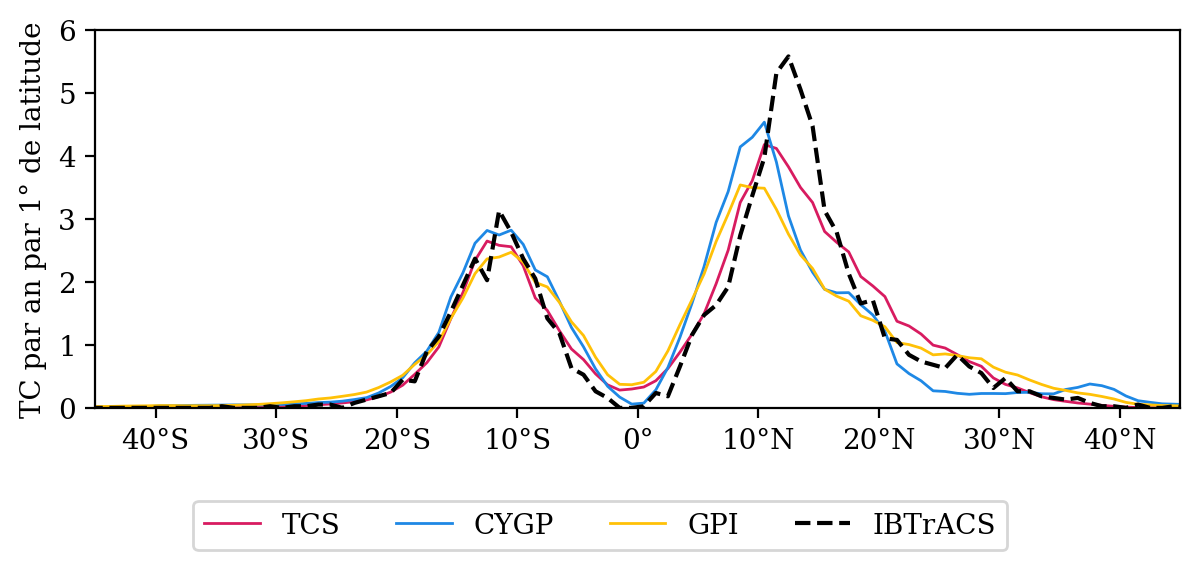
\includegraphics[width=0.8\textwidth]{tcs_cygp_gpi_ibt_zonal_sum_1981_2019.png}
    \caption{Intégrale zonale de la moyenne annuelle du TCS, CYGP et du GPI calculés sur les champs mensuels ERA5 interpolés sur une grille régulière de 1° de
    résolution horizonale, entre 1981 et 2019. Le tracé en tirets indique la distribution méridionale annuelle moyenne des premières observations des systèmes
    IBTrACS renseignés comme tempêtes tropicales ou subtropicales sur la même période et sur la même grille spatiale.}
    \label{fig:tcs_cygp_gpi_zonal}
\end{figure}
%
Comme indiqué par \textcite{menkes_comparison_2012}, qui évaluent ces trois mêmes indices (ainsi que le YGP) sur quatre réanalyses antérieures à ERA5, les trois
indices tendent à surévaluer l'activité cyclonique à proximité de l'équateur, aussi bien dans l'hémisphère nord que dans le sud. Sur ERA5, seul le CYGP atteint
quasiment 0 à l'équateur (\num{0.05} TC par an à exactement 0° par interpolation quadratique, les points de grille les plus proches étant \ang{0.5}S et
\ang{0.5}N), tandis que le TCS et le GPI y simulent respectivement \num{0.3} et \num{0.4} TC par an. Dans l'hémisphère sud, les trois indices ainsi que les
observations sont en bon accord pour ce qui concerne l'amplitude de l'activité méridionale moyenne ainsi que sa position. Le maximum des observations est
atteint à la latitude \ang{11.5}S avec \num{3.13} TC par an. Le TCS, CYGP et le GPI quant à eux ont une latitude du maximum de respectivement \ang{12.5}S,
\ang{10.5}S et \ang{10.5}S. Les trois indices atteignent donc leur maximum aux latitudes directement voisines du maximum d'IBTrACS, de part et d'autre de
celle-ci, l'espacement étant de \ang{1}. Le CYGP simule le pic le plus fort et au plus proche des observations avec \num{2.9} TC par an à la latitude du
maximum, suivi dans l'ordre du TCS (\num{2.7} TC par an) et enfin du GPI (\num{2.5} TC par an). Notons toutefois que, lorsqu'intégré entre \ang{60}S et
l'équateur, le TCS produit l'activité la plus proche des observations, avec \num{26.8} TC par an contre \num{26.1} TC par an dans IBTrACS (voir aussi
\cref{tab:tcs_cygp_gpi}). Les deux autres indices surestiment également l'activité totale de cet hémisphère avec \num{31.9} TC par an pour le CYGP et \num{30.7}
TC par an pour le GPI. En effet, si les trois indices surévaluent l'activité à proximité de l'équateur, le CYGP et le GPI la surestiment également dans les
latitudes plus basses, là où le TCS suit fidèlement IBTrACS. Dans l'hémisphère sud, la cohérence entre les trois indices et les observations est améliorée par
rapport aux résultats obtenus par \textcite{menkes_comparison_2012}, notamment sur ERA-40, distante d'ERA5 de deux générations.

Dans l'hémisphère nord, les performances des trois indices sont nettement plus contrastées. Ni l'amplitude, ni la position du pic d'activité, ni l'étendue
méridionale des trois indices ne correspondent aux observations. Ils présentent tous un biais équatorial plus ou moins prononcé, avec une différence de \ang{4}
pour le GPI et de \ang{2} pour le TCS et le CYGP dans la latitude du maximum. Bien que le CYGP et le TCS partagent la même latitude du maximum, le biais
équatorial du CYGP est distinctement plus prononcé que pour le TCS, ce dernier présentant la meilleure ressemblance avec IBTrACS. Comme pour l'hémisphère sud,
le TCS présente là aussi la meilleure activité totale intégrée entre \ang{0} et \ang{60}N avec un déficit de \num{0.7} TC par an. Le GPI arrive en seconde
position avec un déficit de \num{4.5} TC par an tandis que le CYGP présente un déficit plus conséquent de \num{5.7} TC par an. Le CYGP se distingue également
par un regain d'activité entre \ang{35}N et \ang{40}N, évalué à \num{1.3} TC par an sur cette bande. Ainsi, sur ERA5, les trois indices surestiment l'activité
cyclonique annuelle moyenne dans l'hémisphère sud, et la sous-estiment dans le nord. Le TCS présente toutefois l'activité intégrée la plus proche, ainsi que la
meilleure distribution méridionale.

\subsubsection*{Climatologie mensuelle}

La \cref{fig:tcs_cygp_gpi_clim_mensuel} présente quant à elle la climatologie mensuelle pour les trois indices, évaluée selon le même mode opératoire que pour
la \cref{fig:tcs_cygp_gpi_zonal} ---~à cela près que l'intégration spatiale des indices est réalisée aussi bien en longitude qu'en latitude~--- pour IBTrACS et
pour les 6 bassins océaniques d'intérêt, les frontières de ces derniers étant tracées sur la \cref{fig:bassins_TC} du \cref{chap:chapitre_1}, ainsi que dans la
\cref{sec:papier_appendix_B} du \cref{chap:chapitre_2} \parencite[][documents supplémentaires]{dulac_assessing_2023}. Là encore, les trois indices se
distinguent les uns des autres par des cycles saisonniers aux propriétés variables, bien que tous soient capables de reproduire approximativement la
climatologie observée. 

\begin{figure}[tb]
    \centering
    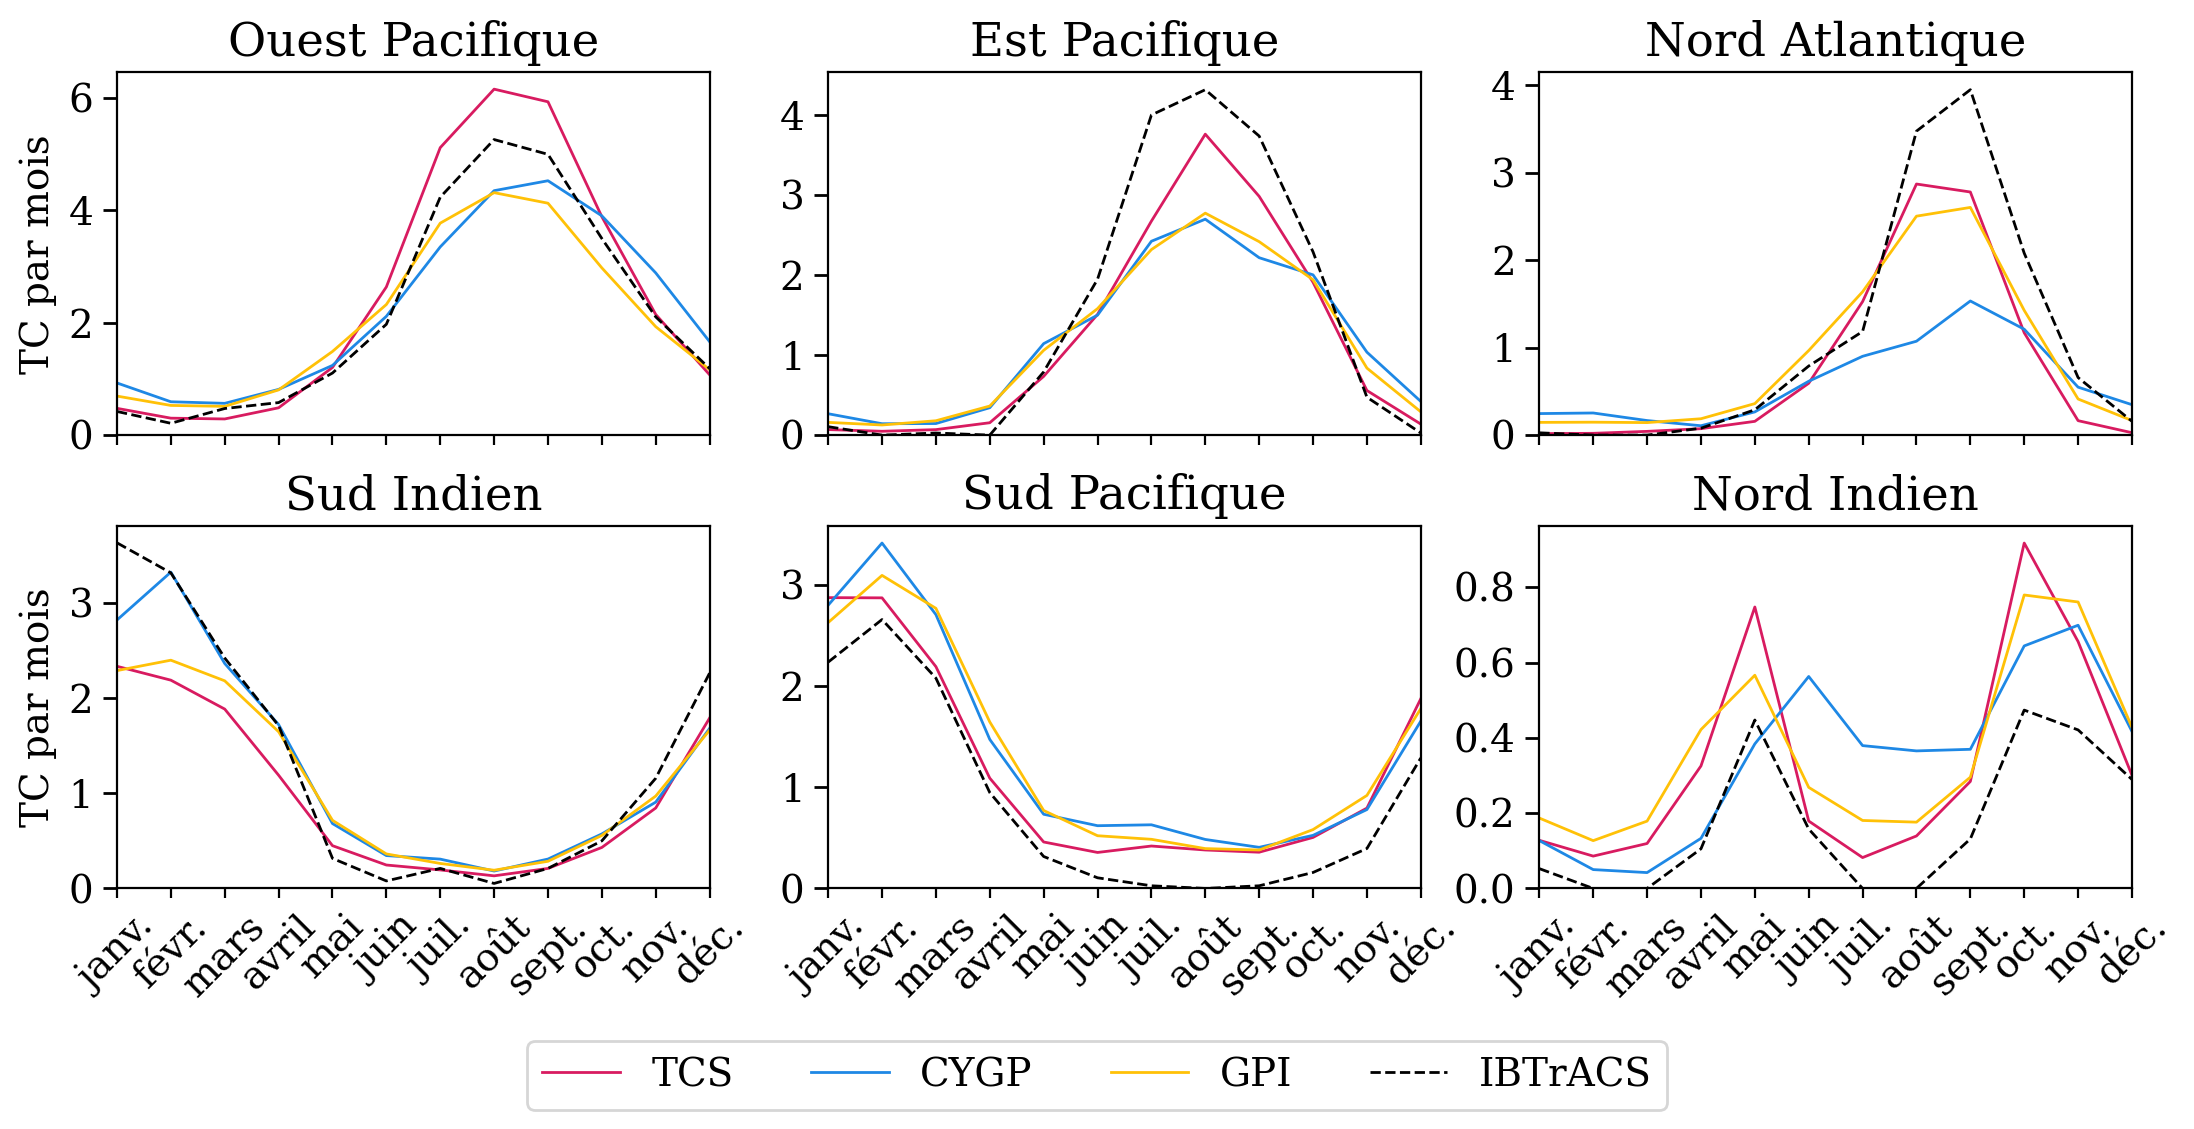
\includegraphics[width=\textwidth]{tcs_cygp_gpi_ibt_clim_mensuel.png}
    \caption{Cycle mensuel de l'activité cyclonique inférée par les trois indices de cyclogénèses définis dans la \cref{sec:tour_horizon_indices} sur
    ERA5 entre 1981 et 2019. Le tracé en tirets noirs indique la climatologie mensuelle observée d'après IBTrACS sur la même période.}
    \label{fig:tcs_cygp_gpi_clim_mensuel}
\end{figure}

Les qualités désirables pour la climatologie mensuelle d'un indice de cyclogénèse à l'échelle régionale sont de pouvoir simuler : la onne saisonnalité, c'est à
dire la bonne étendue temporelle, y compris en minimisant l'activité en dehors de la saison ; la bonne amplitude ; et naturellement le bon nombre de TC moyen
par an. Sur l'ensemble de ces aspects, aucun des trois indices n'apparaît comme clairement supérieur aux autres sur l'ensemble des six bassins d'activité. Les
trois indices capturent correctement la saison cyclonique dans l'ensemble des bassins, à l'exception du CYGP dans le NInd où le pic de la première saison est
indiqué pour le mois de juin plutôt que mai pour les deux autres et dans les observations. Cette caractéristique du CYGP est également notée dans
\textcite{menkes_comparison_2012}, et ne saurait s'expliquer par l'utilisation des précipitations convectives, puisque le YGP présente le même attribut (mais
encore plus prononcé) et trouve par conséquent son origine dans la composante dynamique de l'indice. Le CYGP se démarque par ailleurs du TCS et du GPI à deux
autres reprises : Dans le bassin Nord Atlantique où celui-ci sous-estime très fortement l'amplitude de l'activité (voir aussi \cref{tab:tcs_cygp_gpi}) ; et dans
le bassin Sud-Indien, où il est au contraire le seul à simuler un maximum réaliste au mois de février, bien que la tendance entre janvier et février soit
mauvaise. Le TCS se démarque une de fois de plus comme étant l'indice le plus apte à minimiser l'activité inférée en dehors de la saison cyclonique, bien
qu'elle ne soit tout de même pas négligeable entre juin et octobre dans le bassin SPac, simulant environ \num{0.5} TC par mois, ainsi que dans le NInd entre
juin et août. Par ailleurs, tous les indices surestiment l'activité dans ces deux bassins. Il est toutefois difficile de distinguer la contribution d'IBTrACS de
celle des indices dans ce constat dans la mesure où les observations dans ces bassins y sont moins fiables que dans les autres régions, en particulier dans le
NInd, où les observations sont quasi inexistantes jusqu'au début des années 2000. Les pic d'activités simulés par le TCS dans le WPac, EPac, NAtl et NInd sont
supérieurs à ceux du CYGP et du GPI. Dans le WPac, le TCS dépasse même les observations sur la période juillet~--~août~--~septembre. Dans les deux bassins de
l'hémisphère sud, l'activité inférée par le TCS est au contraire plus faible que pour les deux autres indices (ce qui pour le SPac aboutit à une meilleure
représentation de l'activité observée). Cela se comprend d'une part par le fait, montré dans la section précédente, que le CYGP et le GPI surestiment l'activité
dans l'hémisphère sud tandis qu'ils la sous-estiment dans le nord ---~le TCS étant beaucoup plus proche des observations dans les deux hémisphères~--- et
d'autre part, par la capacité du TCS à capturer plus finement la saison active, en débordant moins que les autres sur la saison creuse. Dans le nord, cela
creuse l'écart du TCS par rapport aux deux autres au cœur de la saison active, tandis qu'il est permis de penser que cette propriété tend au contraire à
compenser l'activité moindre dans le sud. Sans être exempt de tout défaut, le TCS réunit donc, dans l'ensemble, le plus de qualités désirables dans un indice de
cyclogénèse pour simuler la climatologie mensuelle à l'échelle régionale.

\subsection*{Fréquence annuelle et variabilité}

La première partie du \cref{tab:tcs_cygp_gpi} présente la fréquence annuelle moyenne TC dans les six bassins géographiques ainsi que pour chaque hémisphère et à
l'échelle globale. Notons en premier lieu que les trois indices produisent le bon ordre de grandeur de fréquence annuelle à toutes les échelles spatiales, avec
l'exception éventuelle de la sous-estimation du CYGP dans le NAtl, et des trois indices dans le bassin NInd, ce dernier étant probablement dû au manque
d'observations dans la région. Le TCS apparait comme l'indice simulant le nombre moyen annuel de TC le plus proche d'IBTrACS pour \num{5} des \num{8} échelles
spatiales considérées (l'échelle globale ne comptant pas, puisque la fréquence annuelle globale est imposée), à savoir dans le EPac, SPac, NInd et pour les deux
hémisphères. Dans le WPac et le SInd, le TCS est toutefois le plus éloigné de la réalité, et est le seul à produire un surplus dans le WPac, avec $+$\num{3.1}
TC par an par rapport à IBTrACS. Il occupe enfin la 2\ieme~place du classement dans le bassin NAtl, devant le CYGP. Le CYGP quant à lui se démarque dans le WPac
---~bien qu'il ait tendance à simuler une saison légèrement trop tardive, décalée d'environ 1 mois, c.f \cref{fig:tcs_cygp_gpi_clim_mensuel}~--- et dans le
SInd. Enfin, le GPI ne produit la fréquence annuelle la plus proche d'IBTrACS que pour le bassin NAtl, avec cependant un déficit de \num{2.2} TC par an. Dans le
sous-ensemble d'IBTrACS utilisé ici, le ratio de la fréquence annuelle moyenne entre les deux hémisphères est de \num{2.16}. Sans surprise, le TCS en est le
plus proche, avec une différence inférieure à \num{0.01}. Le GPI arrive en seconde position avec \num{1.76} et enfin le CYGP avec \num{1.66}.

\begin{table}[tb]
    \centering
    \caption{Caractéristiques du TCS, du CYGP et du GPI calculés sur ERA5 entre 1981 et 2019 comparé à IBTrACS, par bassin océanique, pour chaque hémisphère
    ainsi qu'à l'échelle globale. Les valeurs en gras renseignent pour chaque colonne l'indice se rapprochant le plus des observations.}
    \begin{tabular}{lrrrrrrrrr}
        \toprule\toprule
        & WPac & EPac & NAtl & SInd & SPac & NInd & NH & SH & Global\\
        \midrule
        \multicolumn{10}{r}{\textbf{Fréquence (TC par an)}}\\
        IBTrACS & \num{26} & \num{17.7} & \num{12.7} & \num{15.9} & \num{10.2} & \num{2} & \num{58.5} & \num{26.1} & \num{84.7}\\
        \midrule
        TCS & \num{29.7} & \textbf{\num{14.6}} & \num{9.4} & \num{11.9} & \textbf{\num{14.2}} & \textbf{\num{4}} & \textbf{\num{57.8}} & \textbf{\num{26.9}} &
        \num{84.7}\\
        CYGP & \textbf{\num{26.9}} & \num{14.3} & \num{7.3} & \textbf{\num{15.2}} & \num{16.2} & \num{4.2} & \num{52.8} & \num{31.9} & \num{84.7}\\
        GPI & \num{29.7} & \num{14} & \textbf{\num{10.7}} & \num{13.5} & \num{16} & \num{4.4} & \num{54} & \num{30.7} & \num{84.7}\\
        \midrule
        \multicolumn{10}{r}{\textbf{Corrélation interannuelle avec IBTrACS}}\\
        TCS & \num{0.03} & \textbf{\num{0.7}} & \num{0.71} & \num{-0.13} & \num{0.35} & --- & \num{0.31} & \num{-0.07} & $<$ \num{0.01} \\
        CYGP & \textbf{\num{0.46}} & \num{0.62} & \num{0.7} & \textbf{\num{-0.13}} & \textbf{\num{0.57}} & --- & \num{0.27} & \textbf{\num{0.05}} & \num{0.01}\\
        GPI & \num{0.06} & \num{0.64} & \textbf{\num{0.79}} & \num{-0.3} & \num{0.39} & --- & \textbf{\num{0.43}} & \num{-0.09} & \textbf{\num{0.17}}\\
        \bottomrule
    \end{tabular}
    \label{tab:tcs_cygp_gpi}
\end{table}

La seconde partie du \cref{tab:tcs_cygp_gpi} présente la corrélation interannuelle des trois indices de cyclogénèses avec IBTrACS pour les mêmes échelles
spatiales. Notons que la variabilité interannuelle est évaluée pour les saisons cycloniques de \num{1981} à \num{2019}, si bien que son calcul fait intervenir
dans l'hémisphère sud les valeurs de l'indice depuis juillet 1980 jusqu'à juin 2019. Cela est valable aussi pour la variabilité à l'échelle globale, évaluée
comme la somme des séries temporelles calculées indépendamment l'une de l'autre sur les deux hémisphères. Précisons également que la variabilité interannuelle
dans IBTrACS pour le bassin NInd est largement composée de \num{0} jusqu'au début des années 2000, raison pour laquelle les corrélations sont omises dans cette
colonne. Là encore, aucun indice ne se distingue clairement des deux autres à toutes les échelles. La capacité des trois indices à produire une variabilité
interannuelle corrélée aux observations est très variable selon les régions du monde et selon les indices. En effet, les trois indices indiquent une corrélation
négative dans le SInd, jusqu'à \num{-0.3} pour le GPI. Dans le WPac, le TCS et le GPI ne présentent aucune corrélation, tandis que le CYGP indique un
coefficient, certes faible mais sensiblement meilleur que pour les deux autres, de \num{0.46}. À l'inverse, dans les bassins EPac et NAtl, les trois indices
indiquent une variabilité interannuelle en phase avec IBTrACS. En effet dans l'EPac, le TCS indique une corrélation de \num{0.7}, suivi du GPI avec \num{0.64}
et enfin du CYGP à \num{0.62}, tandis que le GPI dans le NAtl atteint la plus haute corrélation de \num{0.79} ---~le TCS et le CYGP présentant des performances
honorables d'environ \num{0.7} chacun. Le CYGP se distingue aussi dans le SPac avec une corrélation relativement faible de \num{0.57}, mais meilleure que les
deux autres indices puisque celles-ci valent \num{0.39} et \num{0.35} pour le GPI et le TCS, respectivement. À plus grande échelle, la variabilité interannuelle
des indices dans l'hémisphère nord est plus proche que dans le sud, avec dans le premier cas, entre \num{0.27} pour le CYGP et \num{0.43} pour le GPI, tandis
que dans l'hémisphère sud les trois indices indiquent une corrélation quasi-nulle. À l'échelle globale, seul le GPI indique une très maigre corrélation de
\num{0.17}, les deux autres indices ne présentant une fois de plus aucun lien avec les observations. Séparer le bassin SInd en deux sous-bassins s'avère
bénéfique pour la corrélation interannuelle des trois indices. Spécifiquement, on définit le bassin Sud Ouest Indien (SIndW) entre \ang{20}E et \ang{90}E de
longitude, puis le bassin Sud Est Indien (SIndE), correspondant au bassin australien, entre \ang{90} et \ang{135}E. La limite méridionale demeure inchangée,
entre \ang{0} et \ang{60}S. Ce découpage est plus proche du découpage pratiqué pour la surveillance opérationnelle, comme expliqué dans la
\cref{sec:bassins_saisons} du \cref{chap:chapitre_1}. Dans ce contexte, le TCS présente une corrélation de \num{0.21} et \num{0.22} pour le SIndW et le SIndE
respectivement ; \num{0.37} et \num{0.16} pour le CYGP ; \num{0.27} et \num{0.12} pour le GPI. Par conséquent, et pour la suite des travaux présentés dans ce
document, nous distinguerons toujours les régions SIndW et SIndE.

\begin{figure}[tb]
    \centering
    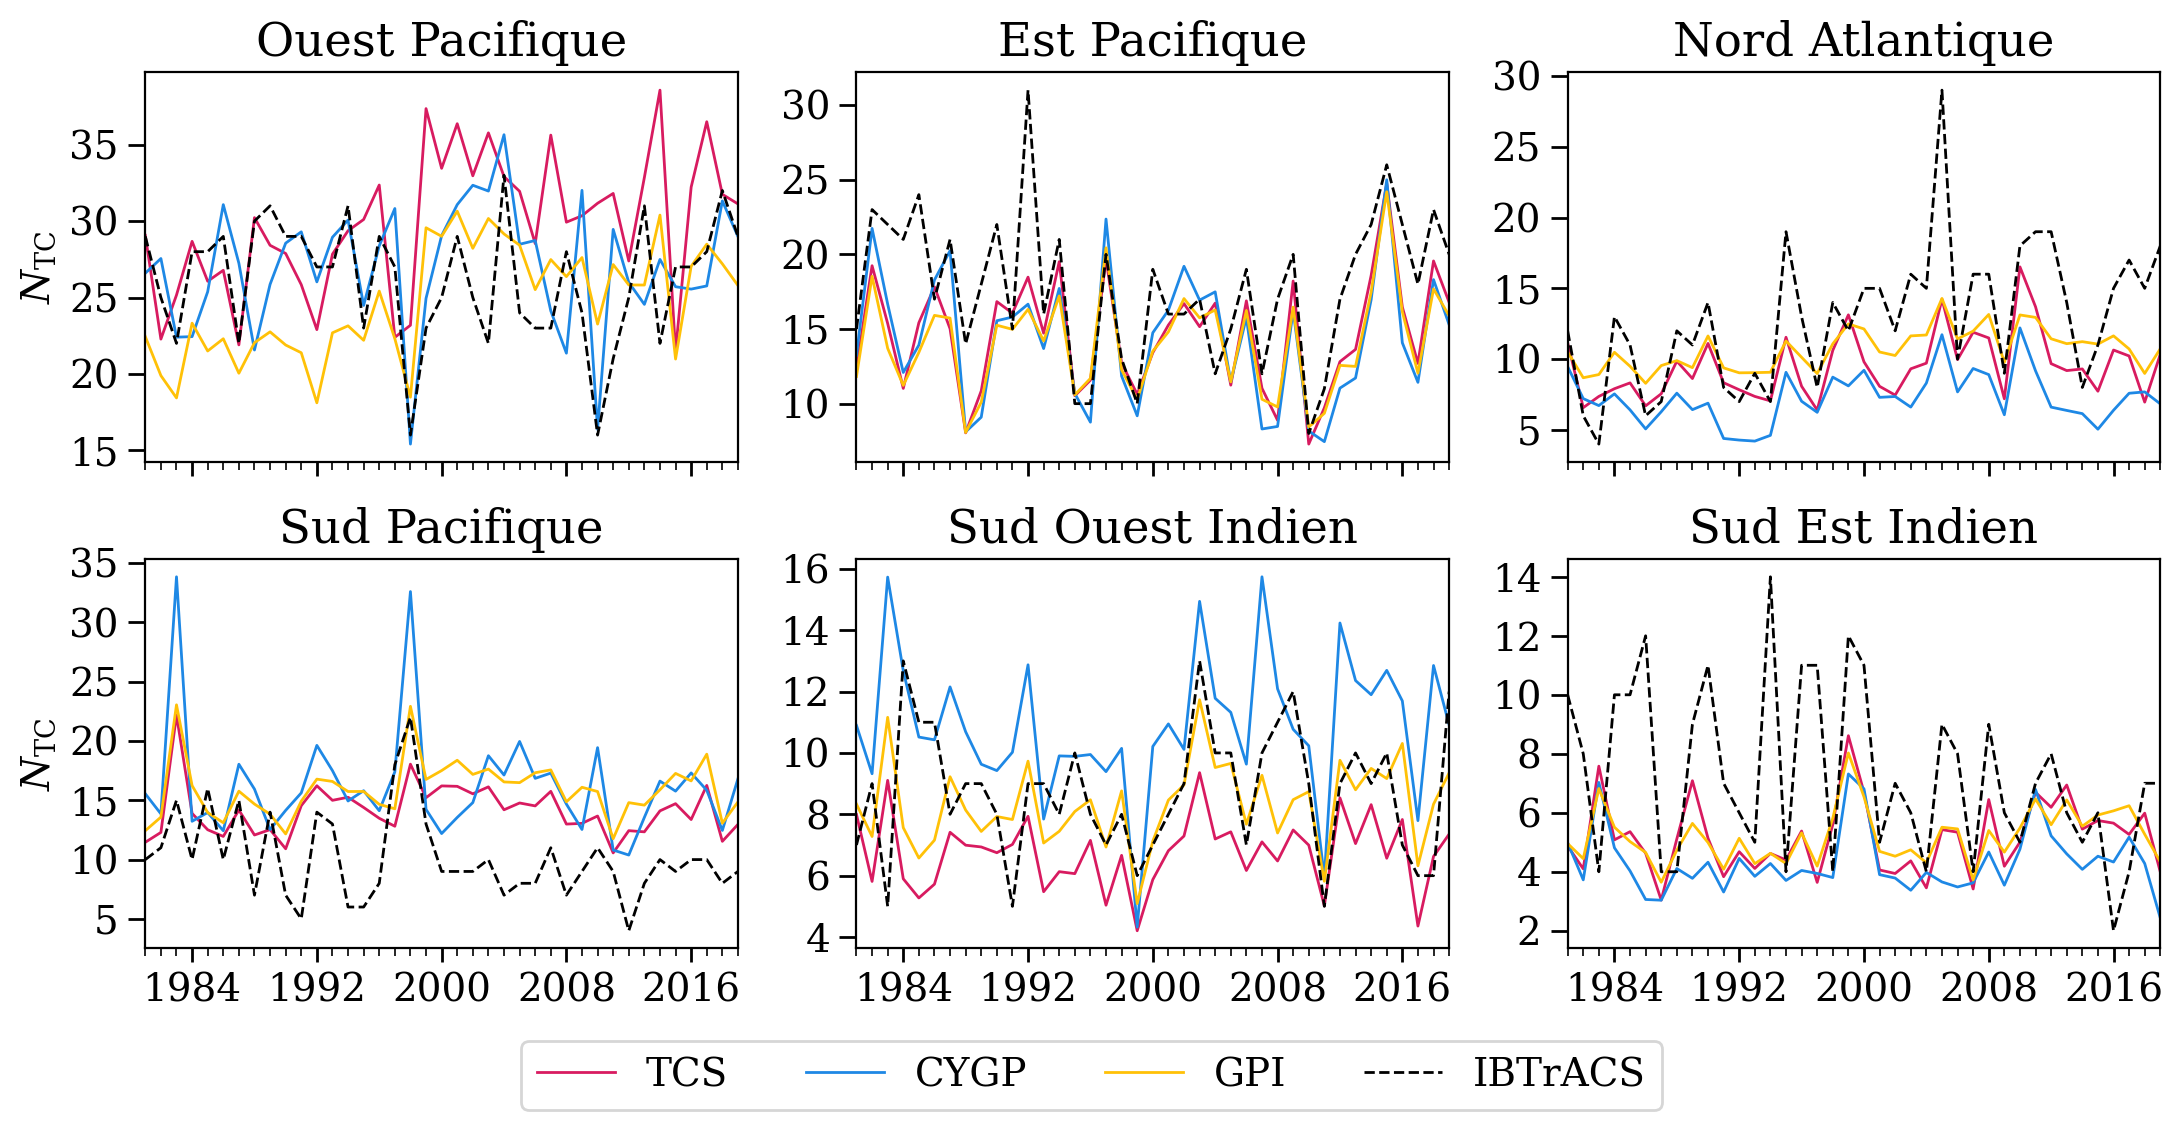
\includegraphics[width=\textwidth]{tcs_cygp_gpi_interannual.png}
    \caption{Variabilité interannuelle entre 1981 et 2019 inférée pour le TCS, le CYGP et le GPI, comparé à IBTrACS.}
    \label{fig:tcs_cygp_gpi_variabilite}
\end{figure}

Enfin, il est important de préciser qu'une bonne corrélation ne présage en rien de la capacité d'un indice à simuler une amplitude réaliste de sa variabilité
interannuelle. La \cref{fig:tcs_cygp_gpi_variabilite} présente les séries temporelles de variabilité interannuelles entre les saisons cycloniques \num{1981} et
\num{2019} dont sont issues les corrélations du \cref{tab:tcs_cygp_gpi}. Dans le bassin NAtl, où la corrélation interannuelle est supérieure à \num{0.7} pour
les indices, l'amplitude de la variabilité inférée est moindre par rapport aux observations. Cela est particulièrement vrai pour le GPI, présentant un
écart-type de \num{1.4} TC contre \num{4.8} TC dans IBTrACS. Le TCS présente une amplitude plus forte que le GPI, mais cette dernière reste toutefois faible,
avec un écart-type de \num{2.3}, soit une dispersion plus de deux fois petite que la dispersion observée. Certains sursauts observés sont cependant capturés par
les trois indices. C'est notamment le cas de l'année \num{1995} et \num{2005}. Dans le Sud Pacifique et Sud Est Indien, le constat est similaire, avec une forte
sous-estimation de l'amplitude à l'exception de certains pics comme pour la saison \num{1998} dans le SPac. Le sursaut d'activité simulé par le CYGP est par
ailleurs anormalement élevé, par rapport aux observations ainsi qu'aux deux autres indices, dépassant \num{32} TC. Cette valeur n'est dépassée qu'en \num{1983}
avec près de \num{34} TC, le GPI et le TCS étant quant à eux en accord sur une valeur de \num{23} TC et \num{22.2} respectivement. Si ces pics notés dans les
trois indices correspondent à un maximum local dans les observations également, la saison ne se démarque toutefois pas des autres saisons. En revanche, le
bassin EPac présente un accord remarquable entre la variabilité simulée et la variabilité observée, avec pour seules exceptions l'année \num{1992}, pic majeur
dans IBTrACS avec \num{31} systèmes, là où les trois indices indiquent entre \num{18.5} TC pour le TCS et \num{16.3} TC pour le GPI. La variabilité inférée par
les indices est, de manière générale, nettement moins proche d'IBTrACS avant l'année \num{1993}, puisque le seul désaccord au delà de cette année \num{2000}.
Notons en effet que la corrélation interannuelle pour le bassin EPac pris à partir de \num{1993} est augmentée d'au moins \num{0.1} par rapport aux valeurs
reinseignées dans le \cref{tab:tcs_cygp_gpi}, atteignant \num{0.81} pour le TCS. Dans l'EPac, SInd (ouest et est), les trois indices présentent des variabilités
extrêmement semblables, mis à part les différences dans la fréquence moyenne dans le SIndW. Les différences sont plus marquées dans le WPac, en particulier
entre le GPI et les deux autres. Le CYGP apparait parfois en opposition du signal indiqué par le TCS et le GPI comme par exemple pour les années \num{1988} et
\num{2007}.

\subsection{Limitations des indices de cyclogénèses}

Les indices de cyclogénèses couramment utilisés dans la littérature et présentés ici présentent une grande capacité à simuler la répartition spatiale et
temporelle de l'activité cyclonique moyenne. Spatialement, les indices présentent un accord important dans l'hémisphère sud, aussi bien entre eux qu'avec les
observations. Dans l'hémisphère nord, la répartition méridionale est plus contrastée et tous les indices présentent un biais équatorial plus ou moins
conséquent. Le TCS se distingue comme le plus apte à simuler cette distribution, ainsi que la répartition de la fréquence annuelle globale entre les deux
hémisphères. De plus, le TCS et le GPI sont tous deux capables de simuler un cycle annuel réaliste dans les 6 bassins océaniques majeurs, tandis que le CYGP
montre des faiblesses dans le NInd et dans le NAtl, où l'activité est fortement sous-estimée, ainsi que dans une mesure bien moindre dans le WPac où avec un
retard d'un mois. Le TCS présente la qualité de discriminer plus finement la saison active de la saison creuse, résultant en une activité cyclonique hors saison
réduite par rapport aux deux autres indices. La fréquence annuelle à l'échelle régionale, ou plus exactement sa proximité avec la fréquence observée, est
variable selon les bassins, mais les trois indices apparaissent comme capables de simuler le bon ordre de grandeur pour chacun des bassins (à l'exception NInd,
probablement en raison du manque de fiabilité des observations dans cette région). Le TCS se démarque toutefois comme produisant la fréquence annuelle la plus
réaliste dans 5 des 8 échelles spatiales considérées.

À l'échelle interannuelle, les performances des trois indices apparaissent comme nettement moins bonnes. À l'exception de certains bassins, tels que le EPac et
le NAtl, la corrélation interannuelle demeure très faible, voire inexistante. De plus, les indices peinent souvent à simuler une amplitude réaliste de cette
variabilité. Ces caractéristiques ne concernent pas seulement la réanalyse ERA5 et sont connues de longue date
\parencite{watterson_seasonal_1995,camargo_tropical_2007,tippett_poisson_2011,menkes_comparison_2012,cavicchia_tropical_2023a}.

\noindent[Rédaction en cours]

%--------------------------------------
\section{Exploration du potentiel prédictif d'un indice à l'échelle saisonnière}

\subsection{Choix du pas d'agrégation temporelle : Mensuel versus saisonnier}

\subsection{Effet de la résolution spatiale et temporelle}\label{sec:resolution_spatiale_temporelle}

\subsection{Activité observée versus modèle ARPEGE}

\subsection{Scores de performances sur la variabilité inter-annuelle}


%--------------------------------------
\section{Synthèse}

\end{document}
